\newpage
\section{Auswertung}
\label{sec:Auswertung}
Die gesmate Messdauer der Hauptmessung Betrug $T=\SI{257100}{\second}$. In dieser Zeit wurden $N_{Start}=3857582$ und $N_{Stop}=738$ Stopsignale gemessen. Dies ergibt eine Eventrate von $f=\frac{N_{Start}}{T}=\SI{15,004\pm0,008}{\hertz}$
\subsection{Wahl der Verzögerungszeit}
Die für zwei unterschiedliche Pulsbreiten wurde die Zählrate in Abhängigkeit von der Verzögerungszeit zwischen beiden Komponenten der Koinzidenzschaltung gemessen. Die Messdauer pro Verzögerungszeit Betrug dabei $T_{mess}=5s$. 
\begin{tabular}
\centering
\caption{Tabelle der Messdaten für die Zählrate in Abhängigkeit von der Verzögerungszeit für eine Pulsbreite von $\SI{18}{\nano\second}$}
\label{tab:18ns}
\begin{tblr}{colspec={c c}}
\toprule
dt[ns] & N \\
\midrule
-26 & 0 \\
-25 & 2 \\
-24 & 8 \\
-22 & 19 \\
-20 & 23 \\
-18 & 35 \\
-16 & 43 \\
-14 & 59 \\
-12 & 61 \\
-10 & 72 \\
-8 & 51 \\
-6 & 61 \\
-4 & 52 \\
-2 & 58 \\
-1 & 35 \\
0 & 45 \\
1 & 63 \\
2 & 68 \\
4 & 53 \\
6 & 39 \\
8 & 40 \\
10 & 24 \\
12 & 16 \\
14 & 6 \\
16 & 3 \\
18 & 1 \\
20 & 0 \\
22 & 0 \\
\bottomrule
\end{tblr}
\end{table}
Die Unsicherheiten können aufgrund der zugrundeliegenden Poissonverteilung aus der Zählrate als $\sigma_N=\sqrt{N}$ berechnet werden.
\begin{figure}
\centering
\includegraphics[width=0.6\textwidth]{plots/Auflösungszeit_18ns}
\caption{Zählrate in Abhängigkeit von der Verzögerungszeit für eine Pulsbreite von $\SI{18}{\nano\second}$.}
\label{fig:18ns}
\end{figure}
\begin{figure}
\centering
\includegraphics[width=0.6\textwidth]{plots/Auflösungszeit_10ns}
\caption{Zählrate in Abhängigkeit von der Verzögerungszeit für eine Pulsbreite von $\SI{10}{\nano\second}$.}
\label{fig:10ns}
\end{figure}
Die resultierenden Ergebnisse sind in den Abbildungen $\ref{fig:18ns}$ und $\ref{fig:10ns}$ dargestellt. 
\begin{tabular}
\centering
\caption{Tabelle der Messdaten für die Zählrate in Abhängigkeit von der Verzögerungszeit für eine Pulsbreite von $\SI{10}{\nano\second}$}
\label{tab:10ns}
\begin{tblr}{colspec={c c}}
\toprule
dt[ns] & N \\
\midrule
-26 & 2 \\
-25 & 1 \\
-24 & 1 \\
-22 & 0 \\
-20 & 0 \\
-18 & 8 \\
-16 & 6 \\
-14 & 11 \\
-12 & 23 \\
-10 & 27 \\
-8 & 53 \\
-6 & 64 \\
-4 & 65 \\
-2 & 60 \\
-1 & 77 \\
0 & 65 \\
1 & 60 \\
2 & 53 \\
4 & 58 \\
6 & 64 \\
8 & 37 \\
10 & 26 \\
12 & 16 \\
14 & 6 \\
16 & 7 \\
18 & 1 \\
20 & 0 \\
22 & 0 \\
\bottomrule
\end{tblr}
\end{table}
Für beide Pulsbreiten wurde die konstante Messrate auf dem sichtbaren Plateau und aus dieser die jeweiligen Halbwertsbreiten $t_{HWB}$ bestimmt. Die Messdaten befinden sich in den Tabellen $\ref{tab:18ns}$ und $\ref{10ns}$. Um diese zu ermitteln wird lineare Interpolation zwischen den beiden einschließenden Punkten der Messung verwendet. Für eine Pulsbreite von $\SI{18}{\nano\second}$ ergibt dies:
\begin{gather}
dt_{18ns,links}=\SI{-19,125}{\nano\second} \\
dt_{18ns,rechts}=\SI{9,47}{\nano\second} \\
t_{HWB,18ns}=\SI{28,59}{\nano\second} 
\end{gather}
Für die Pulsbreite $\SI{10}{\nano\second}$ resultieren die Ergebnisse:
\begin{gather}
dt_{18ns,links}=\SI{-9,696}{\nano\second} \\
dt_{18ns,rechts}=\SI{9,1}{\nano\second} \\
t_{HWB,10ns}=\SI{18,796}{\nano\second} 
\end{gather}
Daraus lässt sich jeweils die Auflösungszeit $\Delta t$ bestimmen:
\begin{gather}
\Delta t_{18ns}=\lvert2*18-t_{HWB,18ns}\rvert=\SI{7,41}{\nano\second} \\
\Delta t_{10ns}=\lvert2*10-t_{HWB,10ns}\rvert=\SI{1,2}{\nano\second}
\end{gather}
Für die Hauptmessung wurde die Pulsbreite $\SI{10}{\nano\second}$ verwendet. Aufgrund der Platzierung des Plateaus wurde hier im folgenden eine Verzögerungszeit von $dt=\SI{2}{\nano\second}$ 
\subsection{Kalibrierung der Kanalzeit}
Um die Kanäle des MCA für die Messung sinnvoll in eine Zerfallsdauer übersetzen zu können wird mit einem Doppelpusgenerator ein Signal mit einer Festgelegten Zeit eingespeist und die betroffenen Kanäle des Analyzers werden gemessen. 
\begin{tabular}
\centering
\caption{Messdaten für die Kalibrierung des MCA}
\label{tab:MCA}
\begin{tblr}{colspec={c c}}
\toprule
t[\mu s] & Kanal
\midrule
0,5 & 4 \\
1 & 15 \\
1,5 & 26;27 \\
2 & 38 \\
2,5 & 49;50 \\
3 & 60;61 \\
3,5 & 72 \\
4 & 83;84 \\
4,5 & 94;95 \\
5 & 106 \\
5,5 & 117;118 \\
6 & 128;129 \\
6,5 & 140;141 \\
7 & 151;152 \\
7,5 & 162;163 \\
8 & 174;175 \\
\bottomrule
\end{tblr}
\end{table}
Bei mehreren betroffenen Kanälen wurde der Mittelwert gebildet. Die korrespondierenden Messwerte finden sich in Tabelle $\ref{tab:MCA}$.
\begin{figure}
\centering
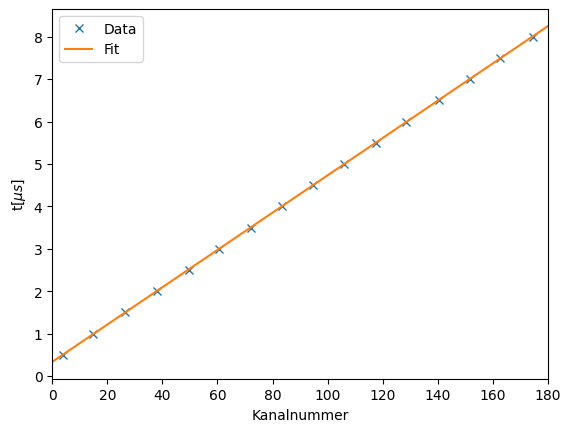
\includegraphics[width=0.6\textwidth]{plots/Kanalkalibrierung}
\caption{Zeit in Abhängigkeit vom angesprochenen Kanal des Multichannel-Analyzers.}
\label{fig:Kanal}
\end{figure}
An diese Messergebnisse kann ein linearer Fit angepasst werden. Die Messung und der zugehörige Fit sind in Abbildung $\ref{fig:Kanal}$ dargestellt. Die Parameter des Fits lauten:
\begin{equation}
t=(0,044\pm4,48*10^{-5})K+(0,331\pm0,0046)
\end{equation}
mit der Zeit $t$ und dem zugehörigen Kanal $K$.
\subsection{Berechnung der Untergrundrate}
Als Zählraten-Experiment unterliegt Zahl der eintreffenden Muonen einer Poissonverteilung. Die Wahrscheinlichkeit, dass bei einer bekannten mittleren Eventrate von $f=\frac{N_{Start}}{T}$ k zusätzliche Myonen während der Suchzeit $T_such$ eintreffen ist daher bestimmt durch
\begin{equation}
P(k)=\frac{(T_{such}f)^k}{k!}e^{T_{such}f}
\end{equation}
und beträgt somit für ein zusätzliches Myon:
\begin{equation}
P(k=1)=0,00012\pm6,113*10^{-8}
\end{equation}
Mittels dieser Wahrscheinlichkeit kann nun die Untergrundrate berechnet werden. Die Untergrundevents teilen sich dabei gleichmäßig auf alle Kanäle auf:
\begin{equation}
U_{poisson}=\frac{N_{Start}*P(1)}{N_{Kanal}}=2,661\pm0,0014
\end{equation}
\subsection{Bestimmung der Zerfallszeit}
Die Messdaten des Multichannel-Analyzers aus der Hauptmessung können mit der dafür angefertigten Fitfunktion auf Zerfallszeiten umgerechnet werden. 
\begin{figure}
\centering
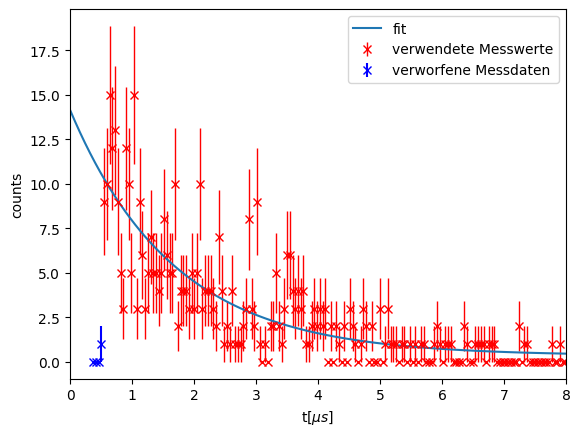
\includegraphics[width=0.8\textwidth]{plots/Hauptmessung}
\caption{Anzahl der gemessenen Ereignisse in abhängigkeit von der Zerfallszeit}
\label{fig:Haupt}
\end{figure}
Die Ergebnisse sind in Abbildung $\ref{fig:Haupt}$ angegeben. An diese Daten kann nun ein Exponentieller Fit der Form:
\begin{equation}
N(t)=N_0e^{-\lambda t}+U_{fit}
\end{equation}
angepasst werden. Dabei wurden die Messwerte aus den ersten vier Kanälen aufgrund der unrealistisch sehr niedrigen Zähllraten vernachlässigt, da diese das Ergebnis stark verfälschen. Dieser liefert mit den vorhandenen Messdaten die Parameter:
\begin{equation}
(12,396\pm0,902)e^{-(0,589\pm0,079)t}+(0,305\pm0,297)
\end{equation}
Aus diesen Parametern kann nun die Lebensdauer zu
\begin{equation}
\tau=\frac{1}{\lambda}=1.7\pm0,23
\end{equation}
bestimmt werden.